\begin{appendices}

%
% The first appendix must be "Self-appraisal".
%
\chapter{Self-appraisal}

<This appendix should contain everything covered by the 'self-appraisal' criterion in the mark scheme. Although there is no length limit for this section, 2---4 pages will normally be sufficient. The format of this section is not prescribed, but you may like to organise your discussion into the following sections and subsections.>

\section{Critical self-evaluation}

\section{Personal reflection and lessons learned}

\section{Legal, social, ethical and professional issues}

<Refer to each of these issues in turn. If one or more is not relevant to your project, you should still explain {\em why} you think it was not relevant.>

\subsection{Legal issues}

\subsection{Social issues}

\subsection{Ethical issues}

\subsection{Professional issues}


%
% Any other appendices you wish to use should come after "Self-appraisal". You can have as many appendices as you like.
%
\chapter{External Material}\label{app:external_material}
<This appendix should provide a brief record of materials used in the solution that are not the student's own work. Such materials might be pieces of codes made available from a research group/company or from the internet, datasets prepared by external users or any preliminary materials/drafts/notes provided by a supervisor. It should be clear what was used as ready-made components and what was developed as part of the project. This appendix should be included even if no external materials were used, in which case a statement to that effect is all that is required.>

\chapter{Visualisation}
\begin{figure}[ht]
    \centering
    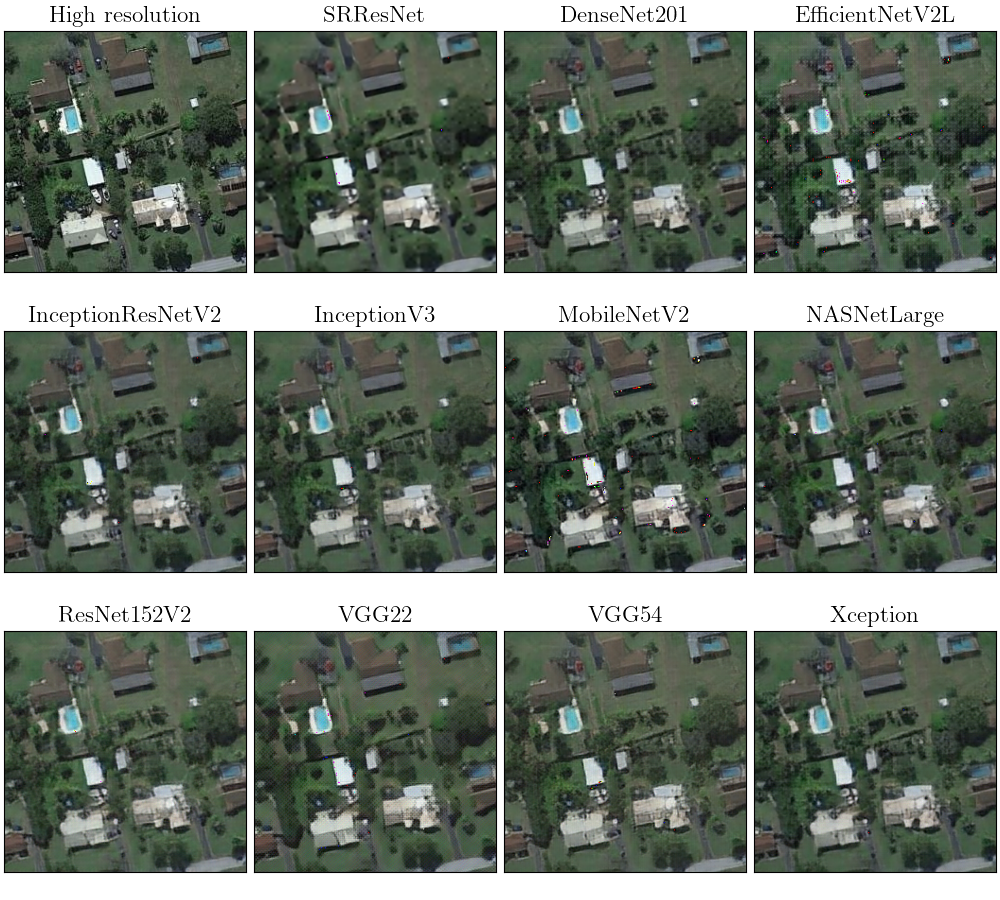
\includegraphics[width=\linewidth]{./assets/model_comparison.png}
    \caption{A comparison using a sample image from the NWPU-RESISC45 test set. The ground truth HR image, SRResNet, and SRGAN models with custom losses are shown.}
    \label{fig:model_comparison}
\end{figure}



%
% Other appendices can be added here following the same pattern as above.
%



\end{appendices}
